\chapter{Glyph-based Poetry Visualization}
\label{chap:additional}

Poems to some may be seen as nothing more than a sequence of words.
To poets however they are a complex system with many links between words (\eg rhyming patterns, and alliteration), many interpretations, and many different ways of reading the same text (there is no indication of exact timing as in music for instance).
A technique called ``close reading'' aims to explore the complexity of such a system through hours of literary analysis devoted to a poem of interest. 
Such readings investigate many variables, including: 
\begin{enumerate}
\item formal information (\eg, lines, and stanzas);
\vspace{-2mm}
\item phonetic information (\eg, meter, intonation, and timing);
\vspace{-2mm}
\item semantic information (\eg, genres, words, repetition, and sentiment); and
\vspace{-2mm}
\item context-driven information (\eg, geographical location, historical period, and political affiliation).
\end{enumerate}

\begin{figure}[h!]
\centering
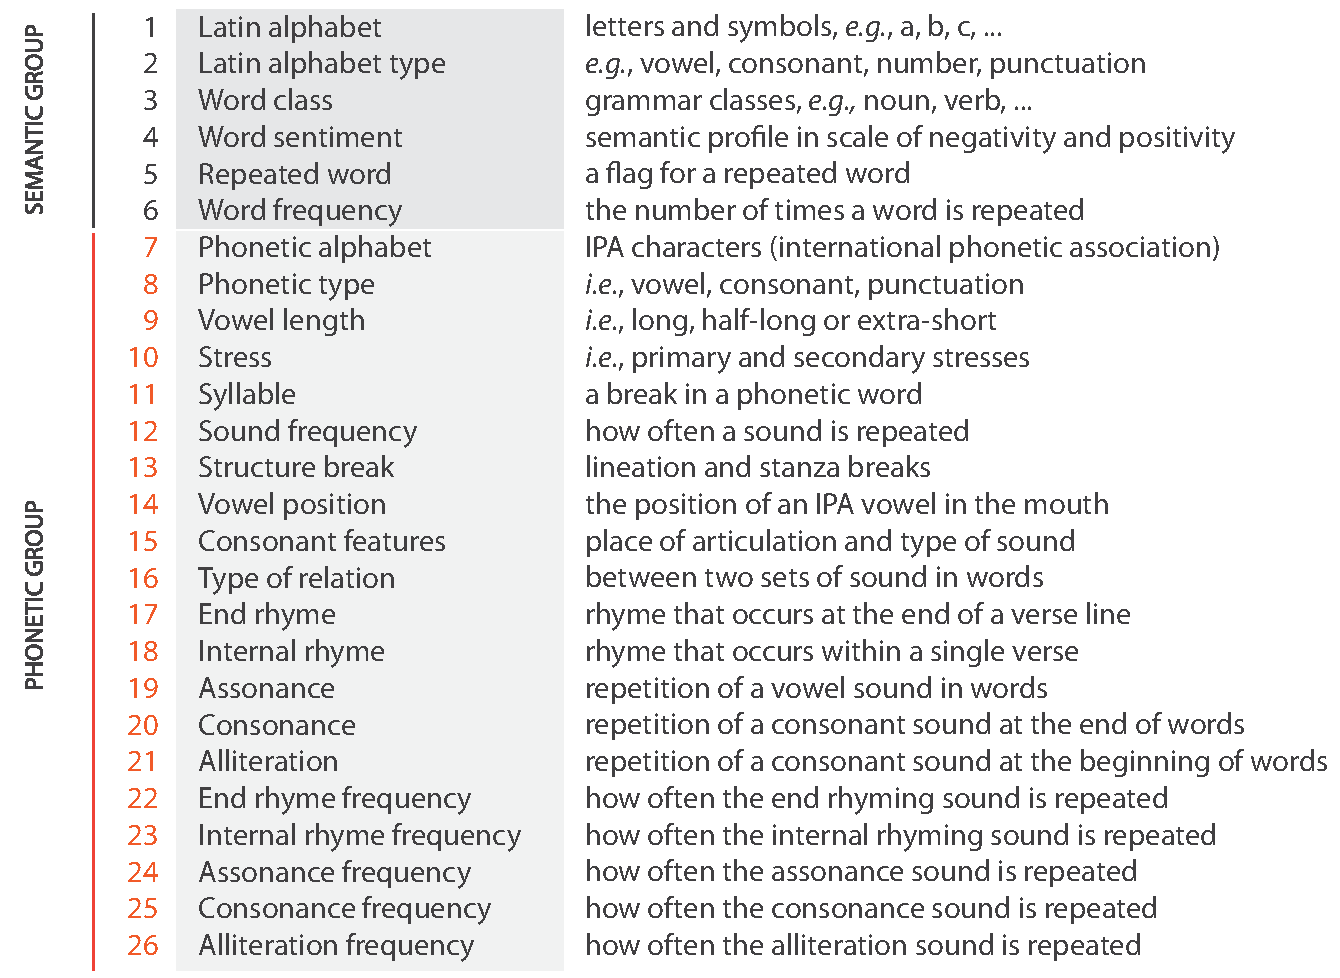
\includegraphics[width=\textwidth]{images/other_glyphs/poem_glyph_vars}
\caption{The six semantic and twenty phonetic variables representing a poem.}
\label{fig:poem_glyph_vars}
\end{figure}


From investigatory discussions with the poetry scholars, thirty-three variables were identified, although only twenty-six were identified as useful for the fifty-two tasks elicited from the scholars using a survey. 
The complete set of variables shown in Figure \ref{fig:poem_glyph_vars} are there to help scholars answer questions such as:
\begin{enumerate}
\item Which of the words in the poem rhyme with each other?
\vspace{-2mm}
\item What is the rhyming pattern in the poem?
\vspace{-2mm}
\item How much sound turbulence is in the poem (changes in the type of sound made through pronunciation of a word)?
\vspace{-2mm}
\item How many of the vowels are rounded vowels?
\vspace{-2mm}
\item Where are the caesurae (line pauses) in the poem?
\vspace{-2mm}
\item How many of the caesurae are masculine caesuras (pause following a stressed syllable)? and
\vspace{-2mm}
\item How many of the caesurae are feminine caesurae (pause following an unstressed syllable)?
\end{enumerate}

The first question that came to mind in the development of this system was how to represent all twenty-six variables. 
Analysis of the tasks that scholars wished to carry out and the variables required to complete each of these tasks showed that not all variables were required for every task. 
Moreover, different scholars were interested in different classes of questions. 
What this means in terms of visual design is that variables may have different levels of importance depending on the task at hand. 
This is in contrast to the work in the previous chapters where there was no variance in the importance of the variables.

The first piece of work investigates the use of knowledge from previous chapters to create a rule-based approach to help systematize glyph design. 
Such a rule-based framework would allow for \emph{controlled} user-defined mappings of the twenty-six poem variables to visual channels.

The second piece of work extends on the first through creation of a static and animated overview glyphs (termed macro glyphs) for each line of a poem to show vowel sound changes/turbulence over time.
This work investigates how statistics can help in the systematization of the animated glyph design, and how design guidelines shown in previous chapters can be applied to aid better memorization of glyphs.

%although seven were removed due to not being suitable to English text (classification between pulmonic (sounds created by air-pressure from the lungs) or non-pulmonic consonants (ejective, implosive or click)), 

\section{Rule-based Mapping for Glyph Creation}

\subsection{Glyph Design}

\begin{figure}[h!]
\centering
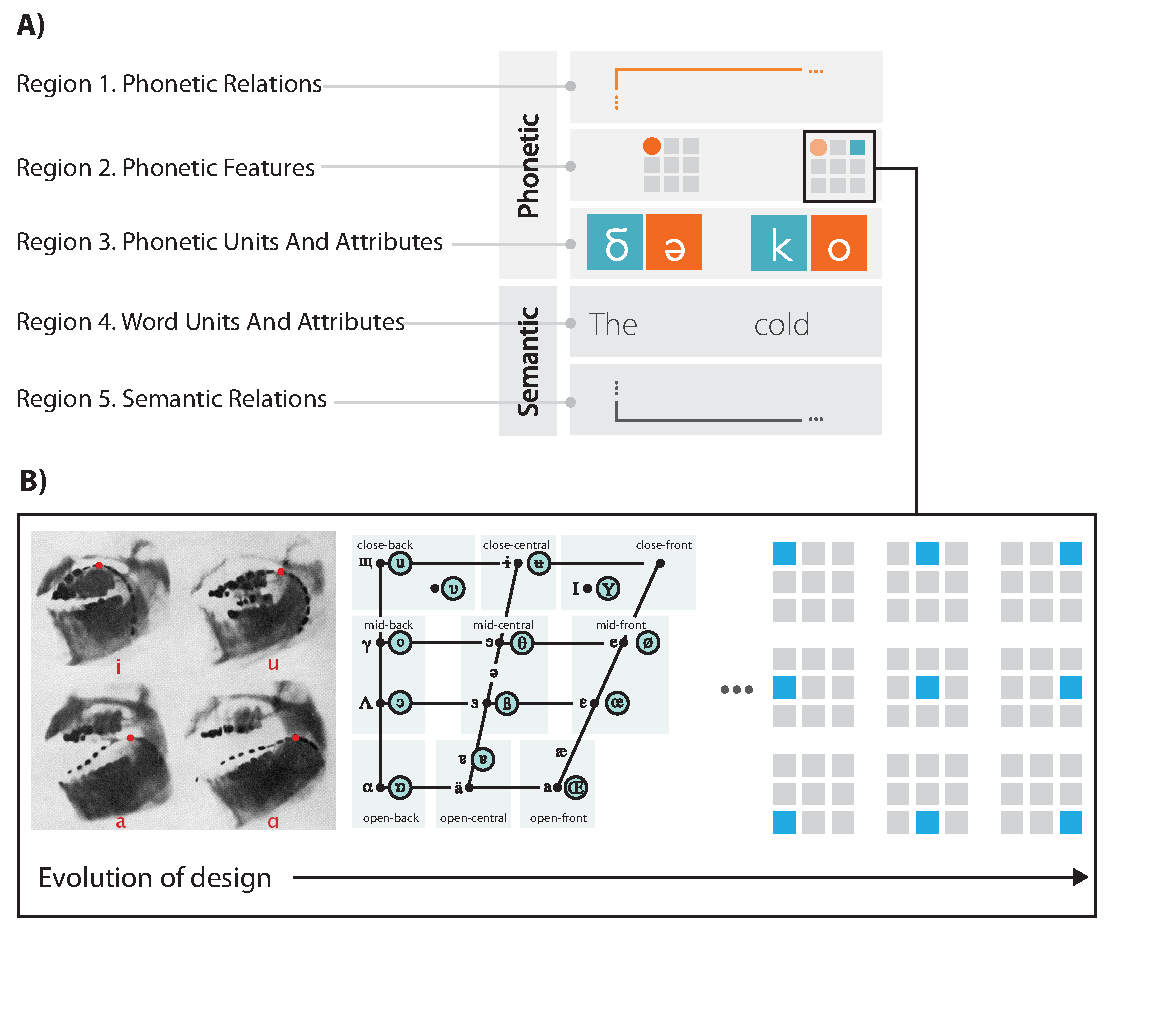
\includegraphics[width=\textwidth]{images/other_glyphs/poem_glyph_design}
\caption{A) The glyph design encompasses five regions to support semantic and phonetic variables listed in Figure \ref{fig:poem_glyph_vars}. 
B) Concrete (top) and abstract (bottom) sub-glyph choices to show how a sound is formed and where the previous sound originated from. It encompasses four pieces of information about: tongue position (close, mid, and open); sound origin (back, central, and front); the transitions by making available the previous position as a more transparent shape; and mouth shape (square or round).}
\label{fig:poem_glyph_design}
\end{figure}

The glyph design is a multi-faceted one with five regions. Two of these regions contain semantic variables, three contain phonetic variables which are:
\begin{enumerate}
\item \textbf{Region 1: Phonetic Relations} between sounds and how they are pronounced \eg, rhyme, end rhyme (line endings that sound the same), alliteration, assonance (repeating vowel sounds), and consonance (repeating consonant sounds). 
\vspace{-2mm}
%This region uses of line colour to represent the different types of relation, and line thickness to represent frequency;
\item \textbf{Region 2: Phonetic Features} showing how the sound is made for vowels and/or consonants \eg, whether the sound is made from the back of the mouth with the tongue up (closed) or down (open) as shown in Figure \ref{fig:poem_glyph_design} B.
\vspace{-2mm}
%This region makes use of pictograms like those shown in Figure \ref{fig:poem_glyph_design} B or symbol shape and colour to represent this data;
\item \textbf{Region 3: Phonetic Units and Attributes} displays the phonetic alphabet, the type (vowel, consonant or punctuation), vowel length, stress (primary or secondary), syllable breaks, sound frequency, and structure break (new line);
\vspace{-2mm}
\item \textbf{Region 4: Word Units and Attributes} displays the word, the type of each component within that word (vowel, consonant, or punctuation), the type of the word (\eg, noun, verb, adjective, adverb, or unknown), and the word sentiment; and
\vspace{-2mm}
\item \textbf{Region 5: Semantic Relations} between words, in this case the repetition of a word and the frequency of repetition.
\end{enumerate}



\subsection{Rule-based Mapping}
Achieving a compromise between the availability of a large number of variables, creating a system that is adept at answering all fifty two tasks, and making the visualization usable and intuitive is a difficult one. 
This problem inspired the creation of a number of rules based on the cognitive science literature that would support an intuitive user interface allowing for changes in the mapping from poem to retinal variables given differences in the tasks being performed.


%rules
Inspired by the ``artificial assistant'' by Mackinlay \etal \cite{mackinlay2007show}, and research highlighted in Chapter \ref{chap:related_work} (\eg, ``semantic mappings'' by Ware \cite{ware2010visual}, and visual ordering by Cleveland and McGill \cite{cleveland1984graphical}, Mackinlay \cite{mackinlay1986automating}, and Heer and Bostock \cite{heer2010crowdsourcing}), and Chapter \ref{chap:glyph-tax}, a number of rules were devised to help automatize the presentation of visual mapping options to the user for the various poetic variables.
These rules are:

\begin{enumerate}
\item \textbf{Rule 1: Spatial separation}. Placing information in the same place every time (visual constancy) enables quicker visual search due to the expectations of users. 
This relates back to \emph{Gestalt} principles discussed in Chapter \ref{chap:related_work} and the law of past experience. 
Figure \ref{fig:poem_glyph_design} A shows five regions with three of these being related to phonetic variables and two related to semantic variables.
By spatially grouping these regions, with all phonetic features at the top and semantic features at the bottom, users will be able to search for variables of interest more quickly.

Formally, this rule encompasses a variable $v$, its group categorization $\Lambda_{group}(v)$, and the region of a visual channel $c$ as $\Theta_{region}(c)$ may be defined as:

\[
\vspace{-1mm}
	S_{R1}(v, c) = \begin{cases}
		1 & \text{if }\Lambda_{group}(v)\text{ is permitted in } \Theta_{region}(c)\\
		0 & \text{otherwise}
	\end{cases}
\]


\item \textbf{Rule 2: Type Compatibility}. As discussed in Chapter \ref{chap:related_work}, some retinal variables are suited better to quantitative data types while others are better suited to qualitative/categorical data. 
Colour hue is better suited to categorical data for example, while it is poorer representation of quantitative data. 

$\Lambda_{type}(v)$ returns five \emph{requirement scores}, $[ \lambda_a, \lambda_s, \lambda_o, \lambda_q, \lambda_r]$, indicating the requirement for $v$ to be associative, selective, ordered, quantitative and relational respectively.
$\Theta_{type}(c)$ returns five \emph{capability scores}, $[ \theta_a, \theta_s, \theta_o, \theta_q, \theta_r]$ indicating the ability of the channel/retinal variable to represent $v$.
All these scores are within the range of [0, 1].
Given these two vector functions, the rule for assessing type compatibility may be defined as:

\[
\vspace{-1mm}
	S_{R2}(v, c) = \frac{\Lambda(v) \bullet \Theta(c)}
	{5 (\lambda_a + \lambda_s + \lambda_o + \lambda_q + \lambda_r)}
\]

\item \textbf{Rule 3: Channel Capacity}. The amount of information that may be represented by a retinal variable is highly dependent on context. 
Context in this case being the resolution available for representation of particular retinal variables.
For instance, if there are three pixels available in total for line width, then there are at most four values (0, 1, 2, and 3 pixels) that may be represented by that line.
This is not considering the error correction that should be applied to minimize error when users read off values.
With four values in a three pixel space, the chance of mistaking 1 pixel with 2 pixels or 2 pixels with 3 is high.
Having a greater number of steps between values would help in error reduction. 
So instead of having four values, we may have two values where there is zero chance of error (0 and 3 pixels). 
However, this greatly limits the channel capacity.
The same is true of colour hue. 
A typical display can render $256^3$ colours (approximately 16.7 million).
The visual system is able to perceive almost all of these colours, but is not always able to tell the difference. 
This is in part due to problems with colour perception discussed in Chapter \ref{chap:related_work} where we showed how colour is perceived relative to its background, so the same colour will look differently depending on context.
Healey \cite{healey1996choosing} and Ware \cite{ware13} suggest that the numbers of distinguishable colours to be used in a visualization should be kept to between five and twelve. 
In this work, each retinal variable was mapped to a numeric value indicating its maximum capacity. 
A simple metric defined below then gave a value of $1$ if the maximum number of values in $v$ ($V_{max}$) could be represented by the lower limit of the retinal variable capacity ($c_{lower}$), $0$ if the minimum number of values in $v$ ($v_{min}$) is greater than the upper limit of the retinal variable capacity ($c_{upper}$), and 0.5 for everything in between.

\[
\vspace{-2mm}
	S_{R3}(v, c) = \begin{cases}
	1 & \text{if }v_{max} \leq c_{lower}\\
	0 & \text{if }v_{min} \geq c_{upper}\\
	0.5 & \text{otherwise}
	\end{cases}
\vspace{-1mm}
\]


\item \textbf{Rule 4: Already in Use}. Too much of anything is often undesirable. If colour hue, colour value, texture, or shape are already in use, using a different retinal variable is encouraged to avoid overloading that particular channel. 
This rule is defined below.

\[
\vspace{-2mm}
	S_{R4}(v, c) = \begin{cases}
	0 & \text{if }$c$\text{ is in use} \\
	1 & \text{otherwise}
	\end{cases}
\vspace{-1mm}
\]

\end{enumerate}

Given that the metrics are normalized to the range $[0,1]$, they may be combined via a simple operation defined below.
\[
\vspace{-1mm}
	S(v, c) = \bigl ( \prod_{i=1}^4 S_{Ri}(v, c) \bigr ) ^{1/4}
\]

A threshold $t$ within the range $[0,1]$ can be set so that for a retinal variable to be available as an option to represent a particular poem variable in the user interface, it must have a score above this threshold. 

\subsection{Poem Viewer}
Poem Viewer brings together the overall visual design with the rule-based mappings to present an easy to use system for poetry scholars. 
The poem visualization and mapping interface are shown in Figure \ref{fig:poem_view_overview}. 
Users are able to change a poem variable to visual representation mapping in Figure \ref{fig:poem_view_overview} A (as shown in Figure \ref{fig:poem_view_overview} B) where the representation will then be updated in Figures \ref{fig:poem_view_overview} C, D and E. 

\begin{figure}[h!]
\centering
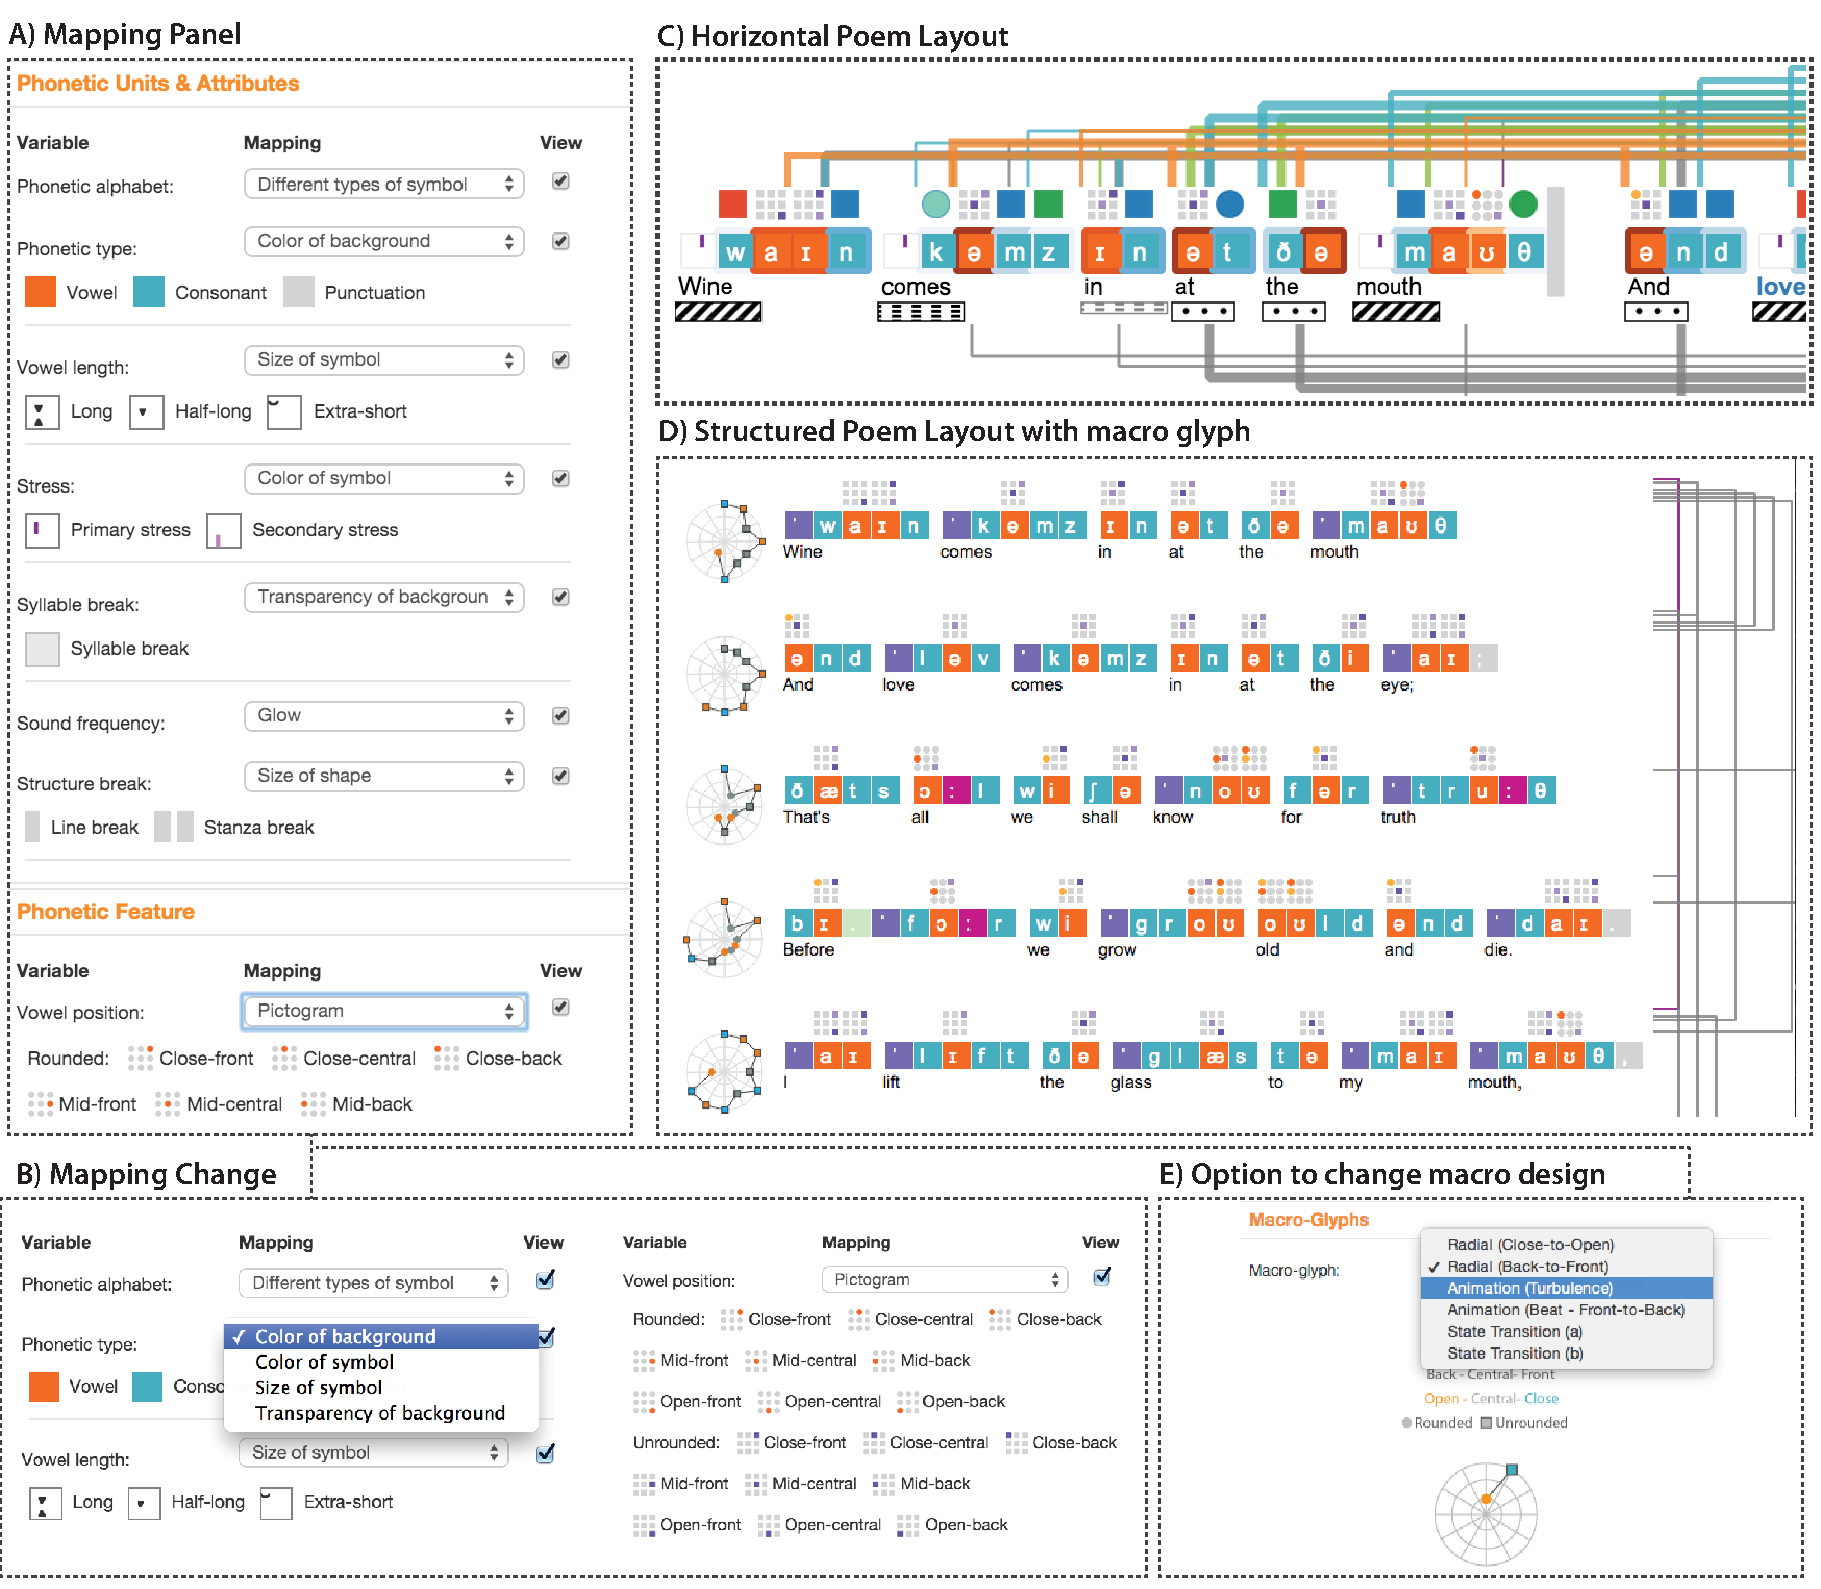
\includegraphics[width=\textwidth]{images/other_glyphs/poemview_overview}
\caption{The Poem Viewer interface.
A) The mapping panel allows users to specify how poem variables are mapped to retinal variables.
B) Changes in mappings are possible through the interface.
C) The poem can be viewed horizontally or in its structured layout in D).
E) An overview of the poem is available showing information such as the long range rhyming patterns.}
\label{fig:poem_view_overview}
\end{figure}

The glyph design process in this work used knowledge presented in Chapter \ref{chap:related_work} along with research conducted in Chapter \ref{chap:glyph-tax} to make the glyph design choices less subjective and more systematic. 
Such an approach made the system easier to build since the number of appropriate visual mappings was significantly reduced from the total possible. 
This rule-based approach also helped avoid pitfalls that could be encountered by allowing too much flexibility in the mapping of poetic variables to unsuitable retinal counterparts.

\section{Macro Glyphs for Poem Turbulence Summaries}

Following the initial PoemViewer system, the poets wished to be able to gain an overview of how the sounds within a poem evolve/flow over time. 
This is termed ``poem turbulence''. 
From the pictorial glyph design in the previous work, it was not easy to follow the changes in sound over time.
The poetry scholars wished to observed patterns in sound changes to determine if certain types of poems have a particular type of ``turbulence pattern''. 
Or, within a poem, are there patterns in sounds between lines.

\subsection{Macro Glyph Design Process}

Similar to Chapter \ref{chap:automacron}, this work proposes the use of ``macros'' (overview representations) to represent many sound transitions as a single glyph.
This approach would solve the issue experienced by poets who wish to be able to see the overall flow of sounds across a line or poem as opposed to reading each pictogram for a vowel or consonant sound one by one.  
However, multiple macro design solutions are possible, all with advantages and disadvantages.
For this type of task, flow can be shown either statically or dynamically. 
In this work we investigate a number of design options, both static and dynamic created using many of the techniques presented in the previous chapters to aid more systematized glyph design. 
The design options are evaluated with a number of poetry scholars to determine which performed better for tasks involved in understanding the sound patterns in poems.  

Of particular relevance to this thesis is the statistical approach taken in the design of the glyphs. 
Thirty-five poems and other English text (books and scientific publications) were analyzed to determine the sounds and transitions between these sounds present in the English language. 
By analyzing not just poems, a more representative view of the transitions that occur in speech within the English language can be obtained.

\begin{figure}[th!]
\centering
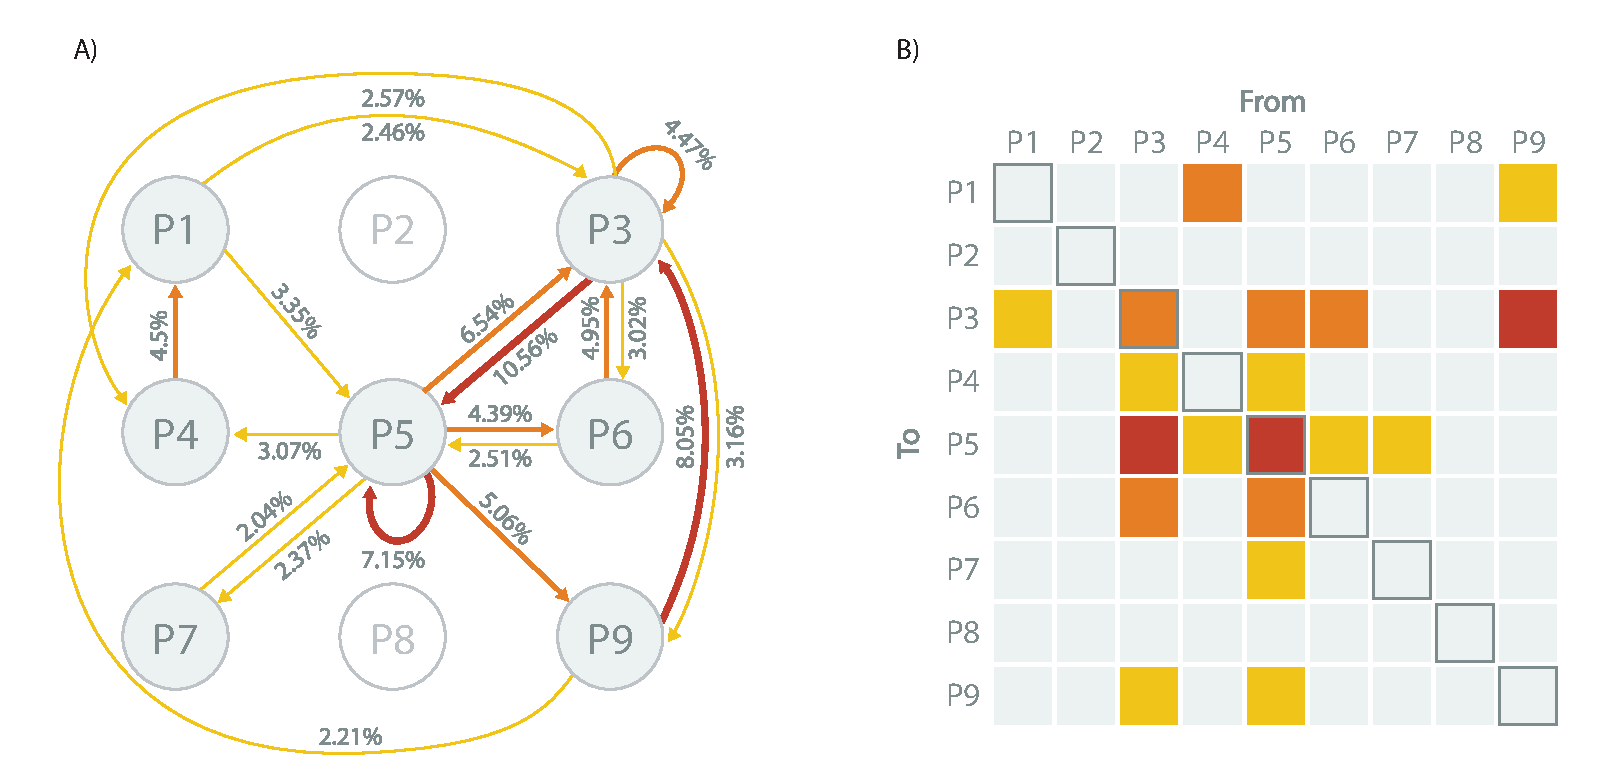
\includegraphics[width=\textwidth]{images/other_glyphs/macro_stats}
\caption{A) Graph showing the different positions of the sounds and tongue position using nodes and the movements between each position using weighted edges. The network shows that two positions are not used in the corpus of data observed.
B) Heat map showing the active areas in the network. 
Both A) and B) are coloured by the number of transitions from one position to another (grey is $f(p_a, p_b) = 0\%$, yellow ($0\%<f(p_a, p_b)< 4\%$), orange ($4\%<=f(p_a, p_b)<7\%$), and red ($f(p_a, p_b)>=7\%$)) where $p_a$ is the \emph{from} position and $p_b$ is the \emph{to} position.}
\label{fig:poem_statistics}
\end{figure}

The statistics gave us answers to the following questions: 
\begin{enumerate}
\item \emph{How many vowel phonemes (sounds that make words sound different from each other) were there per line?} The analysis showed that 84.3\% of lines contain $\leq$12 vowel phonemes and 22 is the maximum number of vowel phonemes;
\item \emph{How many movements were there in the frontness of the sound (back to front)?} The average difference in movement in movement is $\bar\mu=0.7709$ and the standard deviation $\sigma=0.7073$;
\item \emph{How many movements are there between open and closed tongue positions (termed vowel frontness)?} The average difference in movement in movement is $\bar\mu=0.8704$ and the standard deviation $\sigma=0.6699$; and 
\item How many transitions occurred between each position? The results to this are shown in Figure \ref{fig:poem_statistics}.
\end{enumerate}

The \textbf{static radial macro glyph} design benefitted from statistics 1) to 3). 
Initially, the number of spokes or lines representing each vowel phoneme was unknown. 
An initial idea to make the number of lines dynamic would make comparison between lines and positions more difficult. 
A small number of lines may result in the need for many macro glyphs to represent a line.
Conversely, a large number would result in a very densely packed macro glyph that was difficult to visually parse.

Statistic 1) showed that 84.3\% of lines contained twelve vowel phonemes or less while the maximum number of vowel phonemes was twenty-two. 
Twelve fits well with the clock metaphor, and since the temporal aspect is important, familiarity with the clock would make such a glyph easier to interpret. 
The 15.7\% of lines that have more than twelve vowel phonemes would be accommodated through the use of two macro glyphs side by side. 
Alternatively, a twenty-four line glyph that could also fit the clock metaphor, could represent all of the vowel phonemes in lines, however 84.7\% of those lines would occupy less than half of the area of the glyph, and the more densely packed macro glyph would likely be more difficult to interpret.

Statistics 2) and 3) were to inform which axis of the 3x3 vowel sound matrix (vowel frontness and height) would be mapped to which retinal variable. 
The variable with the greatest difference and deviation would be the ideal candidate for a mapping to position. 
Unfortunately there was no outright winner, with vowel frontness having the larger standard deviation and vowel height having the largest average difference.
This resulted in the decision to create both options for evaluation by poets themselves to determine which mapping was more effective.
 
The \textbf{animated macro glyph} benefitted most from statistic 4). 
This statistic, summarized in Figures \ref{fig:poem_statistics} A and B, shows how many transitions there are between across the 3x3 matrix. 
Figure \ref{fig:poem_statistics} A shows a graph depicting all observed transitions with their probability of occurring. Figure \ref{fig:poem_statistics} B presents a matrix-based representation of the graph view. 
It clearly shows how a small subset of all possible transitions between sounds are observed in the data (19/81).
This shows that are large number of movements are not made within the English language (at least according to the sample of English text that was taken). 
Both representations show that positions two and eight have no observed uses.
The greatest activity occurs around positions three and five. 
From such a statistical analysis of the data, we can:
\begin{enumerate}
\item \emph{inform} the design process and implementation of the glyphs through knowing what transitions do and don't happen due to the sounds or transitions not being possible within the language (from this analysis 19/81 transitions are observed in the data). Therefore, instead of creating a glyph that needs to represent all possible transitions between nodes in the graph, many of these hypothetical transitions may be ignored, greatly simplifying the glyph design; and
\item enable the \emph{highlighting} of rare transitions and/or playing down the significance of frequent transitions if poets desired such functionality.
\end{enumerate}

The ability to inform the design process through the statistics greatly simplified the design of the glyphs since the arcs between each position could be better arranged and decluttered.
For example, knowing that there were zero transitions to/from positions two and eight made it possible to inform the animation algorithm to decrease the height of arcs running through positions one and three, and seven and nine. 
Additionally, where connections were uni-directional, the arcs could be less curved than they need to be when visualizing a bi-directional connection. 

\begin{figure}[h!]
\centering
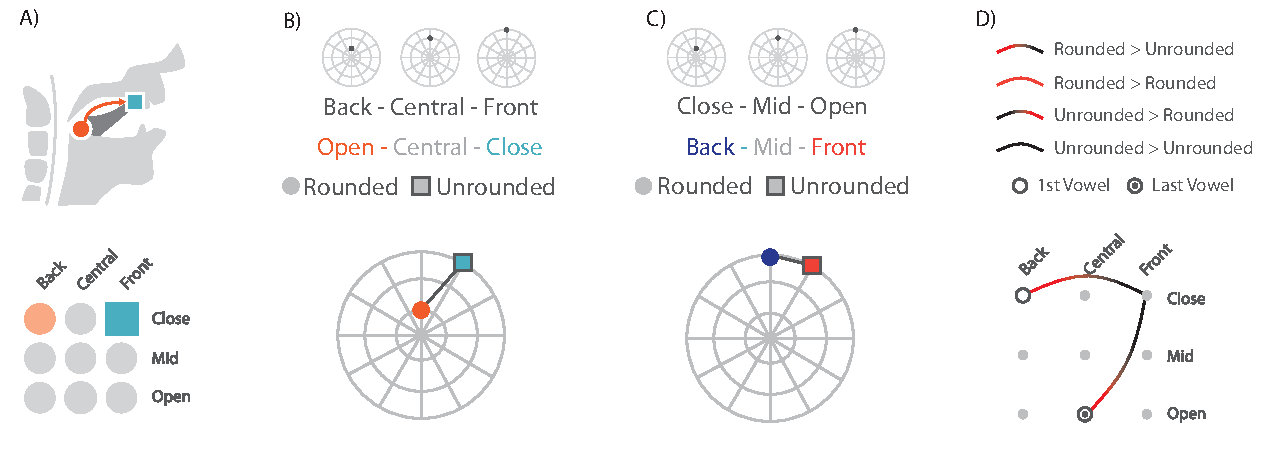
\includegraphics[width=\textwidth]{images/other_glyphs/poem_macro_design}
\caption{Four representations of glyphs showing how a particular sound is formed.
A) This is the original representation of sound movement.
B) A radial layout where time zero is at the top. This representation supports eleven sounds arranged temporally where the difference in distance from the inner to outer rings indicates the change in the sound origin (back to the front of the mouth).
C) An alternative radial layout where the position relates to the tongue being opened, in the middle, or closed.
D) An animated glyph design that shows the flow between points in the 3x3 matrix using animation.}
\label{fig:macro_glyph}
\end{figure}

Figure \ref{fig:macro_glyph} shows the resulting designs of the static radial macro glyphs and the overall schematic for the animated macro glyphs.
 

\begin{figure}[h!]
\centering
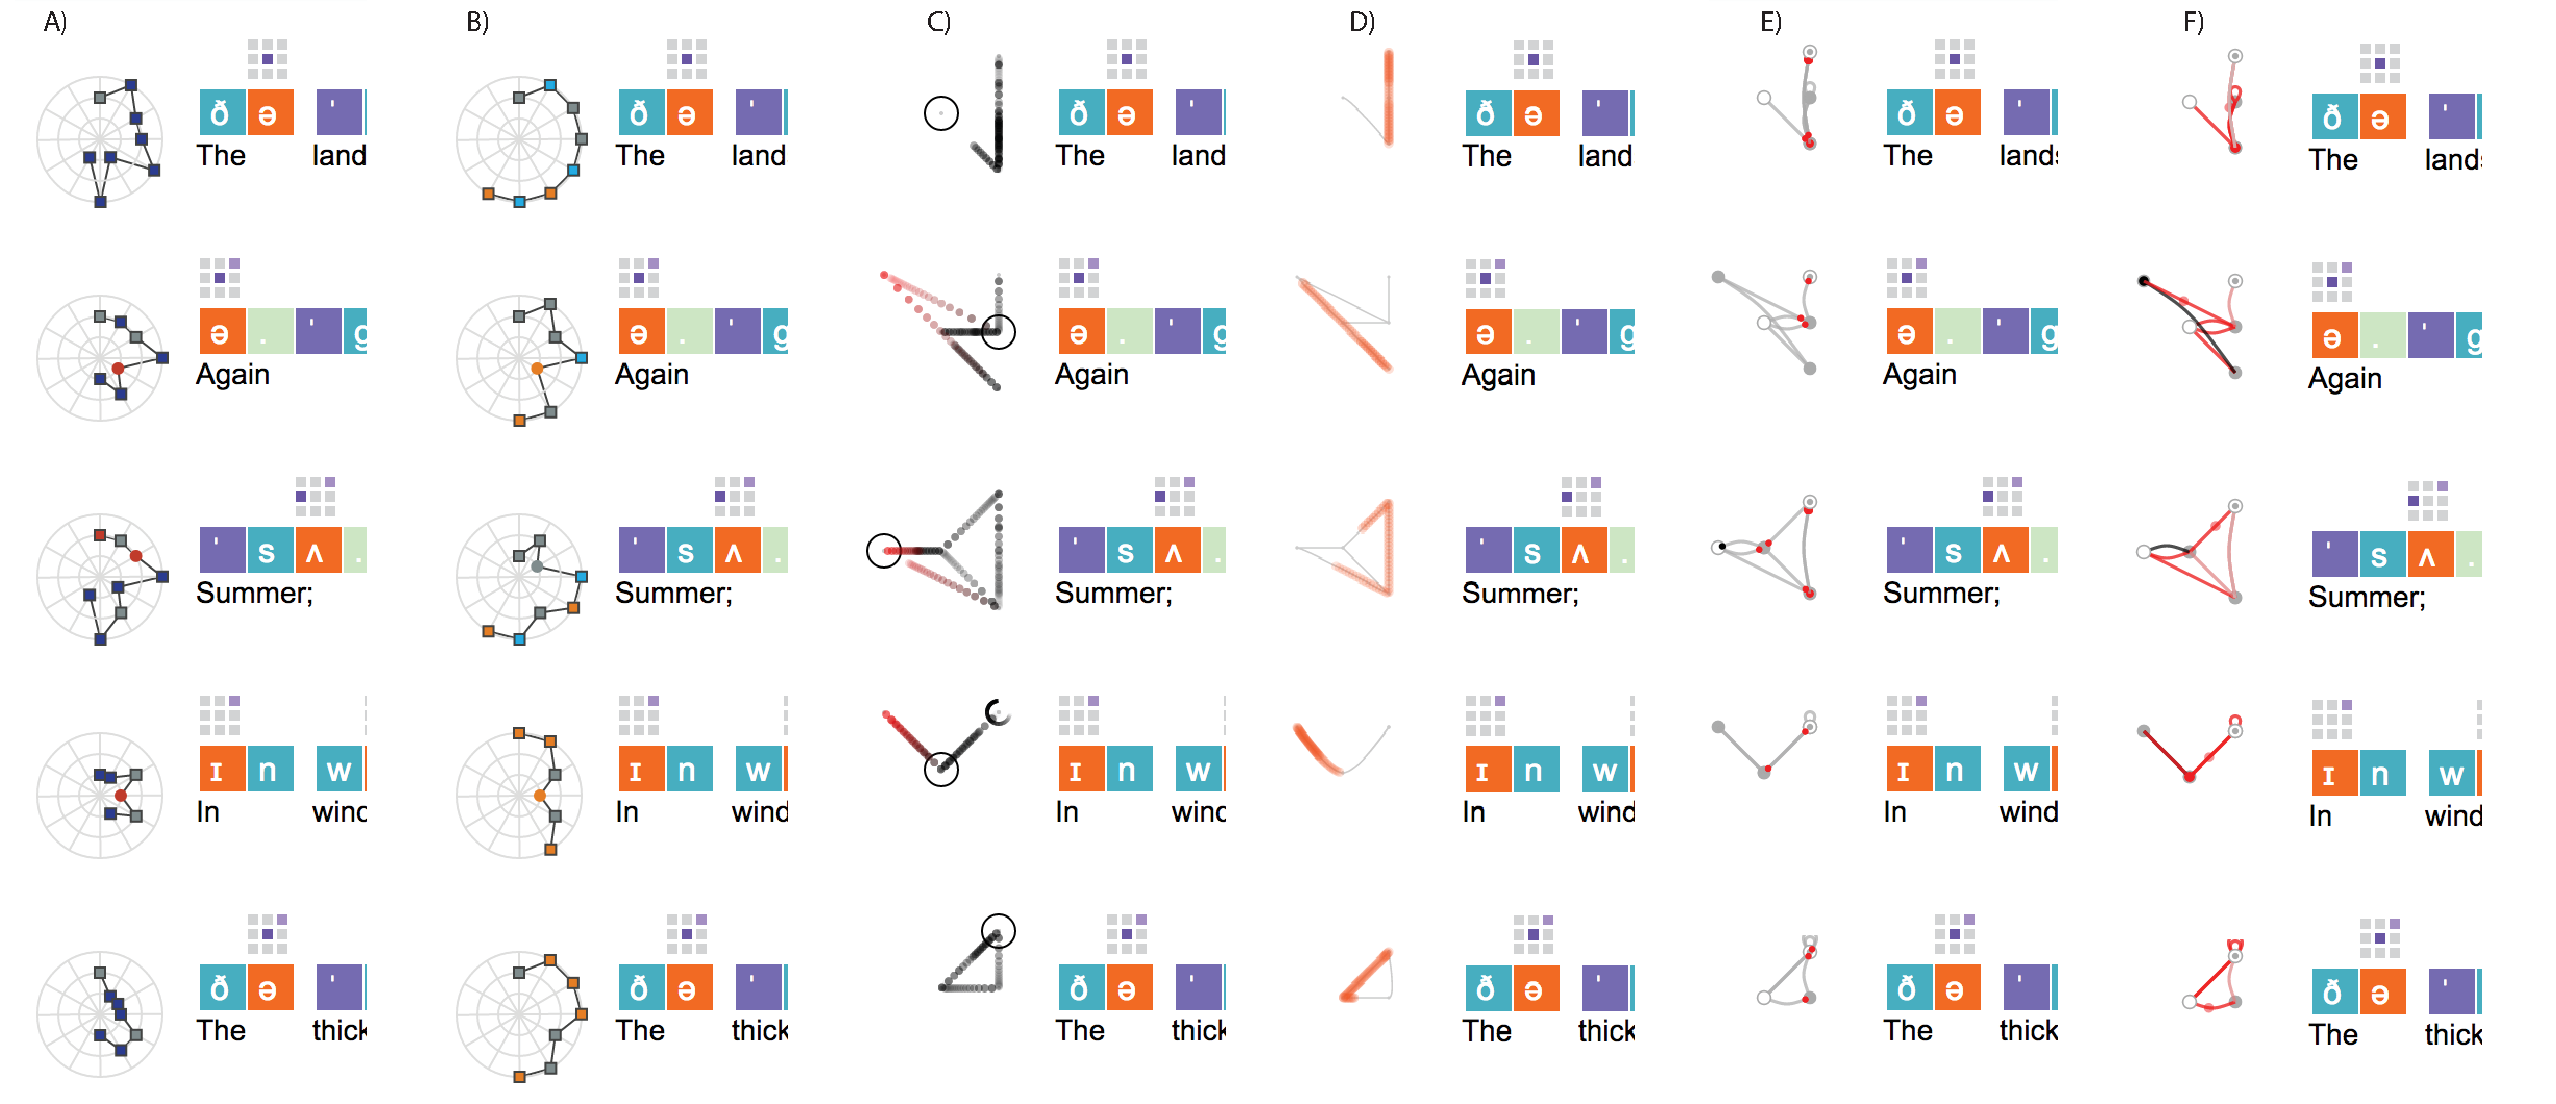
\includegraphics[width=\textwidth]{images/other_glyphs/macros_options}
\caption{Six macro glyphs visualizing five lines of the same poem. 
A) Static radial layout with radial position representing back to front of the mouth.
B) Static radial layout with radial position representing close and open positions of the tongue.
C)-D) Animated transition macro glyphs with trails highlighting previous position. 
E)-F) Animated transition macro glyphs with markers and permanent trails highlighting previous positions.
}
\label{fig:macro_glyph_implementation}
\end{figure}

Figure \ref{fig:macro_glyph_implementation} presents the implementation of the two static macro glyphs, and four variations of the animated macro-glyph, used to visualize five lines of the same poem. 
Due to an understanding that animated glyphs may prove difficult for users wishing to preserve previous transitions, a number of animations were attempted.
Figures \ref{fig:macro_glyph_implementation} C to F represent these different animation strategies to be assessed by expert users.

\subsection{Evaluation}

To evaluate the effectiveness of the macro glyph representation, three postgraduate students in English and French literature, and one Professor of Italian literature were invited to an evaluation session. 
The evaluation consisted of a demonstration of the three designs and the variations of the animated glyphs shown in Figure \ref{fig:macro_glyph_implementation}, followed by a questionnaire consisting of forty-three questions, a discussion, and finally an opportunity to change answers based on the discussions and answers they received.

The responses are summarized as follows:
\begin{itemize}
\item \textbf{Static Radial Macro Glyphs}
\vspace{-1mm}
\begin{enumerate}
\item Both types of radial representations are important to scholars depending on the task;
\vspace{-2mm}
\item Helpful in: a) identification of phonetic patterns among lines; and b) differentiation of dynamics and structures in poems;
\vspace{-2mm}
\item Circles and squares work well for differentiating between rounded and unrounded vowels respectively; and
\vspace{-2mm}
\item The logological link between the colours used and say open (orange) or closed (cyan) tongue made remembering the colour coding an easier process.
\end{enumerate}
\vspace{-2mm}
\item \textbf{Animated Transitions}
\vspace{-1mm}
\begin{enumerate}
\item Entertaining to watch;
\vspace{-2mm}
\item Intuitive to use when observing the general flow but after some time, the temporal ordering is lost; and
\vspace{-2mm}
\item Opacity as a tool for encoding frequencies is helpful but it can present ambiguity;
\end{enumerate}
\vspace{-2mm}
\item \textbf{Static Transitions with Temporal Highlight}
\vspace{-1mm}
\begin{enumerate}
\vspace{-2mm}
\item Similar to the \emph{Animated Transitions}, it is intuitive, but the ability to track is lost after some observation time;
\vspace{-2mm}
\item Residual line patterns show direction and frequency well, but temporal ordering is not shown; and
\vspace{-2mm}
\item The moving highlight is helpful but not enough to enable the remembering of temporal ordering.
\vspace{-2mm}
\end{enumerate}
\end{itemize}

Although the animated macro glyphs were entertaining for the users and did contribute to the analysis of the poem, the most useful macro glyphs for determining the relations between lines of poems were the static representations. 
The issues with animation were understood in advance of this work, in particular the problems with depicting temporal information, however they still proved useful for depicting overall flow of information. 

\section{Summary}

This chapter served to show how some of the systematization techniques presented in Chapter \ref{chap:strategies} could be applied to glyph design for poetry.

The first part of this chapter showed how the use of design principles based on cognitive science knowledge can help systematize the choice of retinal variables presented to users as possible mappings for poetic variables. 
This was published in the Computer Graphics Forum in 2013 in a publication by Abdul-Rahman \etal named Rule-based Visual Mappings -- with a Case Study on Poetry Visualization \cite{CGF:Abd2013a}. 

The second piece of work showed how statistical analysis of the data can help in the glyph design process. 
This work was published as a short paper in 2014 in a publication by Abdul-Rahman \etal named Comparing Three Designs of Macro-Glyphs for Poetry Visualization \cite{CGF:abdul-rahman14-sp}. 
